\begin{figure}[H]
	\centering
	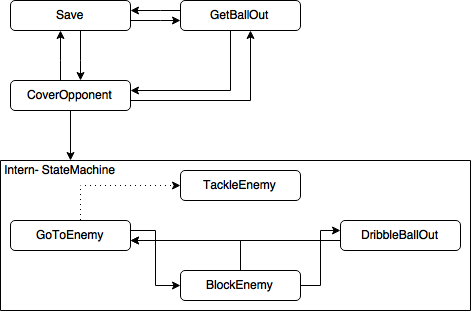
\includegraphics[width=\ScaleIfNeeded]{Grafiken/KI/defender/defender.png}
	\caption{State-Automat des Verteidigers}
	\label{State-Automat des Verteidigers}
\end{figure}
Das folgende Kapitel beschreibt die Funktionsweise und den Prozess zur Erstellung der Rolle des Verteidigers.

\subsubsection{Vorgehensweise}
\begin{figure}[H]
	\centering
	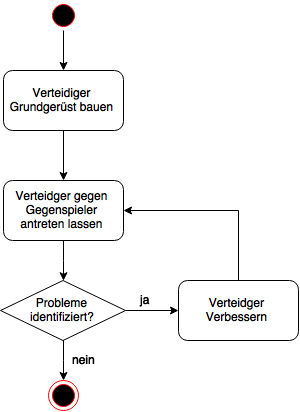
\includegraphics[width=\ScaleIfNeeded]{Grafiken/KI/defender/vorgehensweise.png}
	\caption{Vorgehensweise zur Entwicklung des Verteidigers}
	\label{Vorgehensweise-Verteidigers}
\end{figure}
Der in Abbildung \ref{Vorgehensweise-Verteidgers} dargestellte Prozess ist der Anforderung geschuldet zu einem m"oglichst fr"uhen Zeitpunkt bereits einen funktionierenden Spieler auf das Feld schicken zu k"onnen. Deswegen wurde ein iterativer Prozess gew"ahlt, dabei wird initial ein einfaches Grundger"ust entwickelt welches anschlie"senden Zyklisch verbessert werden kann. Der Prozess kann verlassen werden, wenn keine Zeit mehr f"ur Verbesserungen vorhanden ist, oder keine weiteren Probleme mit der Logik des Verteidigers gefunden werden k"onnen.\\
\\
\subsubsection{Use-Cases}
\begin{figure}[H]
	\centering
	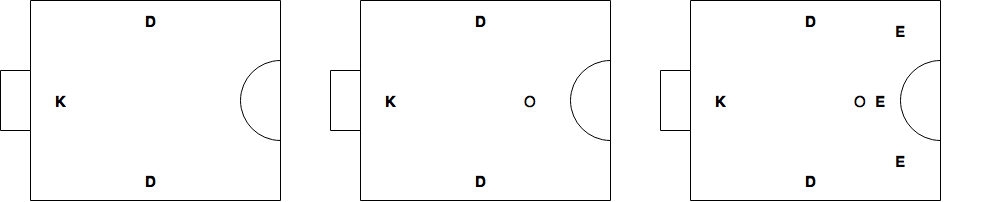
\includegraphics[width=\ScaleIfNeeded]{Grafiken/KI/defender/useCases.png}
	\caption{Die Use-Cases des Verteidigers}
	\label{Usecases-Verteidigers}
\end{figure}

F"ur den Verteidiger wurden die in Abbildung \ref{Usecases-Verteidigers} ermittelten Use-Cases definiert. Dabei gilt zu beachten, dass diese nicht den Anspruch haben alle m"oglichen F"alle abzubilden, sich aber auf einige wenige wichtige zu reduzieren. Dieses Vorgehen ist der Anforderung des einfachen Grundger"ustet geschuldet. F"uer die Use-Cases wurde ferner die idealisierende Annahme getroffen, dass auf der eigenen Spielfeldseite nur Verteidiger existieren. Ferner wurde dem gegnerischen Spieler eine h"ohere Priorit"at zugeteilt als dem Ball, die Annahme hierbei ist, dass der Ball durch den gegnerische Spieler in das Spielfeld getragen wird. Sollte der Ball frei sein und ein gegnerischer Spieler auf der eigenen Feldh"alfte sein, bewegt sich dieser auf den Ball zu, da er von dem Verteidiger gedeckt wird, sollten diese gleichzeitig bei dem Ball ankommen, die daraus resultierende Situation ist dann wieder der erst genannten gleich.

paragraph{UseCase: Spielgeschehen auf anderer Spielh"alfte}
Weder der Ball noch Gegnerische Spieler befinden sich auf der eigenen Spielh"alfte.
paragraph{UseCase: Ball in eigener Spielh"alfte}
Der Ball jedoch keine gegnerischen Spieler befinden sich auf der eigenen Spielh"alfte.
paragraph{UseCase: Gegner (mit Ball) in eigener Spielh"alfte}
Gegnerische Spieler befinden sich auf dem Spielfeld. Dabei ist es unerheblich ob der Ball ebenfalls mit auf dem Spielfeld ist.
